% Options for packages loaded elsewhere
% Options for packages loaded elsewhere
\PassOptionsToPackage{unicode}{hyperref}
\PassOptionsToPackage{hyphens}{url}
\PassOptionsToPackage{dvipsnames,svgnames,x11names}{xcolor}
%
\documentclass[
  letterpaper,
  DIV=11,
  numbers=noendperiod]{scrartcl}
\usepackage{xcolor}
\usepackage{amsmath,amssymb}
\setcounter{secnumdepth}{-\maxdimen} % remove section numbering
\usepackage{iftex}
\ifPDFTeX
  \usepackage[T1]{fontenc}
  \usepackage[utf8]{inputenc}
  \usepackage{textcomp} % provide euro and other symbols
\else % if luatex or xetex
  \usepackage{unicode-math} % this also loads fontspec
  \defaultfontfeatures{Scale=MatchLowercase}
  \defaultfontfeatures[\rmfamily]{Ligatures=TeX,Scale=1}
\fi
\usepackage{lmodern}
\ifPDFTeX\else
  % xetex/luatex font selection
\fi
% Use upquote if available, for straight quotes in verbatim environments
\IfFileExists{upquote.sty}{\usepackage{upquote}}{}
\IfFileExists{microtype.sty}{% use microtype if available
  \usepackage[]{microtype}
  \UseMicrotypeSet[protrusion]{basicmath} % disable protrusion for tt fonts
}{}
\makeatletter
\@ifundefined{KOMAClassName}{% if non-KOMA class
  \IfFileExists{parskip.sty}{%
    \usepackage{parskip}
  }{% else
    \setlength{\parindent}{0pt}
    \setlength{\parskip}{6pt plus 2pt minus 1pt}}
}{% if KOMA class
  \KOMAoptions{parskip=half}}
\makeatother
% Make \paragraph and \subparagraph free-standing
\makeatletter
\ifx\paragraph\undefined\else
  \let\oldparagraph\paragraph
  \renewcommand{\paragraph}{
    \@ifstar
      \xxxParagraphStar
      \xxxParagraphNoStar
  }
  \newcommand{\xxxParagraphStar}[1]{\oldparagraph*{#1}\mbox{}}
  \newcommand{\xxxParagraphNoStar}[1]{\oldparagraph{#1}\mbox{}}
\fi
\ifx\subparagraph\undefined\else
  \let\oldsubparagraph\subparagraph
  \renewcommand{\subparagraph}{
    \@ifstar
      \xxxSubParagraphStar
      \xxxSubParagraphNoStar
  }
  \newcommand{\xxxSubParagraphStar}[1]{\oldsubparagraph*{#1}\mbox{}}
  \newcommand{\xxxSubParagraphNoStar}[1]{\oldsubparagraph{#1}\mbox{}}
\fi
\makeatother


\usepackage{longtable,booktabs,array}
\usepackage{calc} % for calculating minipage widths
% Correct order of tables after \paragraph or \subparagraph
\usepackage{etoolbox}
\makeatletter
\patchcmd\longtable{\par}{\if@noskipsec\mbox{}\fi\par}{}{}
\makeatother
% Allow footnotes in longtable head/foot
\IfFileExists{footnotehyper.sty}{\usepackage{footnotehyper}}{\usepackage{footnote}}
\makesavenoteenv{longtable}
\usepackage{graphicx}
\makeatletter
\newsavebox\pandoc@box
\newcommand*\pandocbounded[1]{% scales image to fit in text height/width
  \sbox\pandoc@box{#1}%
  \Gscale@div\@tempa{\textheight}{\dimexpr\ht\pandoc@box+\dp\pandoc@box\relax}%
  \Gscale@div\@tempb{\linewidth}{\wd\pandoc@box}%
  \ifdim\@tempb\p@<\@tempa\p@\let\@tempa\@tempb\fi% select the smaller of both
  \ifdim\@tempa\p@<\p@\scalebox{\@tempa}{\usebox\pandoc@box}%
  \else\usebox{\pandoc@box}%
  \fi%
}
% Set default figure placement to htbp
\def\fps@figure{htbp}
\makeatother





\setlength{\emergencystretch}{3em} % prevent overfull lines

\providecommand{\tightlist}{%
  \setlength{\itemsep}{0pt}\setlength{\parskip}{0pt}}



 


\KOMAoption{captions}{tableheading}
\makeatletter
\@ifpackageloaded{caption}{}{\usepackage{caption}}
\AtBeginDocument{%
\ifdefined\contentsname
  \renewcommand*\contentsname{Table of contents}
\else
  \newcommand\contentsname{Table of contents}
\fi
\ifdefined\listfigurename
  \renewcommand*\listfigurename{List of Figures}
\else
  \newcommand\listfigurename{List of Figures}
\fi
\ifdefined\listtablename
  \renewcommand*\listtablename{List of Tables}
\else
  \newcommand\listtablename{List of Tables}
\fi
\ifdefined\figurename
  \renewcommand*\figurename{Figure}
\else
  \newcommand\figurename{Figure}
\fi
\ifdefined\tablename
  \renewcommand*\tablename{Table}
\else
  \newcommand\tablename{Table}
\fi
}
\@ifpackageloaded{float}{}{\usepackage{float}}
\floatstyle{ruled}
\@ifundefined{c@chapter}{\newfloat{codelisting}{h}{lop}}{\newfloat{codelisting}{h}{lop}[chapter]}
\floatname{codelisting}{Listing}
\newcommand*\listoflistings{\listof{codelisting}{List of Listings}}
\makeatother
\makeatletter
\makeatother
\makeatletter
\@ifpackageloaded{caption}{}{\usepackage{caption}}
\@ifpackageloaded{subcaption}{}{\usepackage{subcaption}}
\makeatother
\usepackage{bookmark}
\IfFileExists{xurl.sty}{\usepackage{xurl}}{} % add URL line breaks if available
\urlstyle{same}
\hypersetup{
  pdftitle={The Geometry of Prediction, Part I},
  colorlinks=true,
  linkcolor={blue},
  filecolor={Maroon},
  citecolor={Blue},
  urlcolor={Blue},
  pdfcreator={LaTeX via pandoc}}


\title{The Geometry of Prediction, Part I}
\author{}
\date{2025-09-15}
\begin{document}
\maketitle


\section{Part 1}\label{part-1}

I recently read
\href{https://x.com/abeirami/status/1963206009393930569}{this} tweet by
my friend, Ahmad Beirami. My approach to concentration inequalities has
been quite utilitarian, and Ahmad's tweet confirmed to me that I am
missing out on some deep geometric intuition in statistics. This has led
me to revisit some primitives of statistics with which I have long had
merely a pragmatic alliance -- among them the cumulant generating
function, the Chernoff bound, and exponential families -- with the hope
of forging a firmer friendship.

This note will be a preposterously overlong account of the Chernoff
bound -- we will endeavour to understand

Long term, I want to explain why the geometry that we discuss here bears
on estimation theory and online algortihms. The second case is
especially rremarkable, as it shows that we can use statistical ideas in
entirely adversarial scenarios.

I don't wish to get too bogged down in technical details. All the
(in)equalities that follow hold under the mild assumption that they
hold.

\section{Exponential families}\label{exponential-families}

Let's begin with a quick recap of exponential families. These are
parametric statistical models that are computationally and theoretically
favorable, for geometric reasons that will become clear in a moment.

In its natural form, a parametric density \(p_\eta\) is an exponential
family if it has the form
\[p_\eta(x) = p(x) e^{\langle \eta, T(x)\rangle - A(\eta)}\]

Exponential families have many nice properties, including the following

\begin{itemize}
\tightlist
\item
  1 \(\E_{p_\eta} [T(x)] = \nabla A |_\eta\)
\item
  2 \(\Cov_\eta(T(x)) = \nabla^2 A |_\eta\)
\item
  3 \(\E_\eta[e^{\lambda T(x)}] = A(\eta + \lambda) - A(\eta)\)
\item
  4 Given data \(x_1, ... x_n \sim p_\eta\), the MLE for \(eta\),
  \(\hat{\eta}\) is satisfies
  \(\nabla_\eta A(\hat\eta) = \sum_i T(x_i)/n\)
\item
  5 \(KL(p_\eta || p_\lambda) = D_A(\lambda || \eta)\) where \(D_A\) is
  the Bregman divergence under \(A\).
\end{itemize}

These plain lemmas, which can be verified by simple computation, breed
copiously amongst themselves to produce theorems that reveal the
geometry that underlies so much of classical statistics. We'll
scrutinize their progeny later.

For now, however, let us simply notice that, for any base (univariate)
density \(p\), we can define an exponential family by multiplying it by
\(e^{\lambda x}\) and normalizing appropriately:
\[p_\lambda(x) = e^{\lambda x}p(x)/E_p[e^{\lambda x}] = e^{\lambda x - \log \E [e^{\lambda X}]}p(x)\]
so that \(A(\lambda) = \psi(\lambda) = \log \E [e^{\lambda X}]\) and
\(\eta = \lambda\). Thus, whenever we linearly tilt a density, the
C.G.F. enters the stage merely as a normalizing constant. However, in
its capacity as the log-partition function of the so-called Esscher
transform , the C.G.F. acquires an interesting role in defining the
geometry of \(\lambda\)-space

If \(P\) is a measure (as opposed to a density), we can define the
tilted distribution through the Radon-Nikodym derivative
\(\frac{dP_\lambda}{dP} = e^{\lambda x - \psi(\lambda)}\). In this note,
one can rest assured that essentially nothing is lost by considering
this to be a somewhat ostentatious rewrite of the definitional statement
\(p_\lambda(x)/p(x) = e^{\lambda x - \psi(\lambda)}\) .

\section{The Chernoff Bound}\label{the-chernoff-bound}

Here is how the Chernoff argument typically runs in a Master's class. We
have an arbitrary random variable, \(X \sim P\), and we wish to bound
its tail probability, \[\Pr[X > t] \ ; \ t > \E_P[X]\]

We begin by mercilessly mocking the feeble bounds produced by Markov and
Chebyshev -- they retire, dejected. The professor now pulls the
following rabbit out of his or her hat:
\[\mathrm{Pr}[X \geq t] = \inf_\lambda \mathrm{Pr}[e^{\lambda X} \geq e^{\lambda t}] \leq \inf_\lambda e^{- \lambda t + \log \E[e^{\lambda X}]]} = e^{-I(t)} \]

Where \(I\) is dubbed the rate function. Together, the class cranks out
pages of calculation to get supertight binomial tail bounds, or possibly
characterize subgaussian or subexponential random variables. Meanwhile,
the rabbit scampers away into a nearby shrub, never to reappear.

Why did exponentiating magically make Markov's inequality good again?
One may dimly perceive that exponentiation pushes us towards the case of
two point masses, where Markov is tight. But, to me, the precise nature
of this optimization remains elusive.

In order to improve our understanding, we'll prove the Chernoff bound
three different ways, with a special focus on understanding where the
slack in the inequality comes from.

\subsubsection{Proof 2: Circumscribe}\label{proof-2-circumscribe}

As a starting point towards making the Chernoff derivation look less
miraculous, here's one rewrite of the standard proof, using the
numerical inequality \(1\{x \geq t\} \leq e^{\lambda(x - t)}\) for any
\(\lambda > 0\):

\[\Pr[X \geq t] = \E[1\{X \geq t}] = \E[\inf_\lambda e^{\lambda (X - t)}] =  \leq \inf_\lambda \E[e^{\lambda (X - t)}] = \inf_\lambda e^{\psi(\lambda) - \lambda t} = e^{-I(t)}\]

So exponentiating and applying Markov's inequality is the same as
inscribing the tail-indicators induced by \(X\) in an exponential, and
then choosing their rates (\(\lambda\)) to optimize this surrogate on
average over \(X\). In this chain, the slack is in \emph{moving the
infinum out of the expectation}. The looseness of the Chernoff bound is
exactly the \(L^1(P)\) of the looseness of the numerical inequality.

\begin{figure}[H]

{\centering 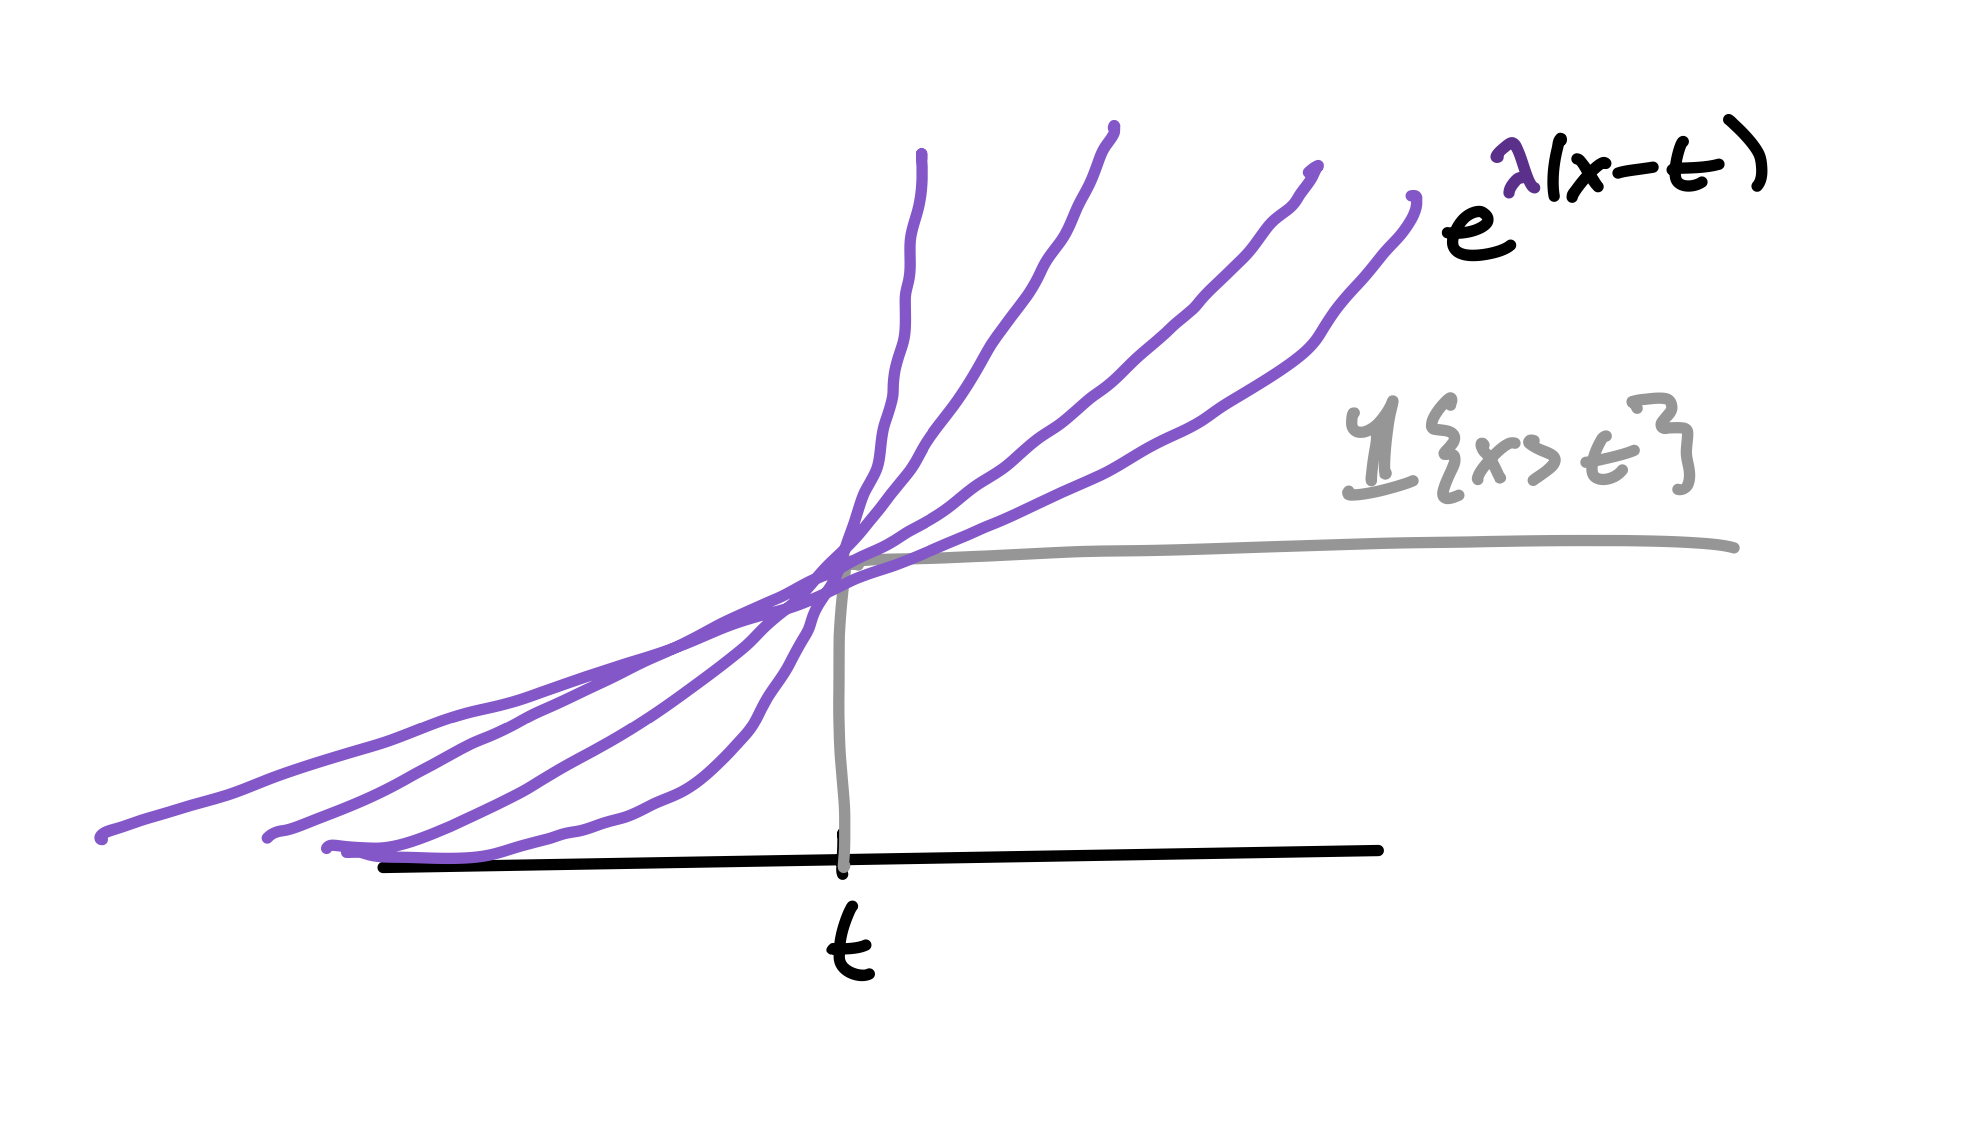
\includegraphics[width=5.20833in,height=\textheight,keepaspectratio]{circumscribe.png}

}

\caption{We can produce an exponential upper bound for the step function
for every rate \(\lambda > 0\). The best upper bound is the one with
smallest \(L^1(P)\) norm.}

\end{figure}%

Incidentally, what we have just seen is that we can recreate
\(\Pr[X \geq t]\) by taking the lower \(\lambda\)-envelope of the
\(t\)-curves \(\psi(\lambda) - \lambda t\) as we sweep
\(\lambda \in [0, \infty]\).

\subsubsection{Proof 3: Tilt}\label{proof-3-tilt}

This time, we will write the tail as an importance-weighted expectation
under the distribution \(P_\lambda\) that satisfies
\(\frac{dP_\lambda}{dP}(x) = e^{\lambda x - \log E[e^{\lambda X}]}\).
For any \(\lambda > 0\), we have

\[\Pr[X \geq t] = \E[1\{X \geq t\}] = \E_{P_\lambda}[\frac{dP}{dP_\lambda}1\{X \geq t\}]\]
\[ \leq e^{- \lambda t + \psi(\lambda)}\Pr_{P_\lambda}[X \geq t]\]

This argument makes the call to Markov explicit, reminding us that all
Markov does is bound the probability of the upper tail by 1. So what
we're doing when we apply the Chernoff method is linearly \emph{tilting}
the base measure \(P\) according to some slope \(\lambda\) and bounding
the tilted tail by \(1\). In doing this, we incur an additional term,
\(e^{-\lambda t + \psi(\lambda)}\), which is optimized by setting the
derivative to zero: \(\psi'(\lambda^*) = t\). By the properties of
exponential families, this actually tells us that, at the optimal tilt,
\(\lambda^*\) \[\E_{P_{\lambda^*}}[X] = \psi'(\lambda^*) = t\] That is,
\(\lambda^*\) is the (unique) tilt that fixes the tilted mean to be
\(t\)!

What is \(e^{-I(t)} = e^{-\lambda^* t + \psi(\lambda^*)}\) ? Well
\[KL(P_{\lambda^*} || P) = \lambda^* \E_{P_{\lambda^*}}[X] - \psi(\lambda) = I(t)\]

This is a little better. The Chernoff bound is going to linearly tilt
\(P\) until the tilted mean is \(t\), and then pay for doing so with
\(e^{-I(t)} = e^{-D(P_{\lambda^*} || P)}\). So the more we have to
linearly tilt \(P\) to have the event \(t\) be unsurprising, the tighter
our tail bound is.

Here's a pithy phrasing for the bound, as bonus. we take the MLE
estimate for \(\lambda\) among the family of linear tilts of \(P\) under
the observation \(x = t\), and see how far it is from \(P\) in KL
divergence (i.e.~in the Fisher-Information metric). This can be seen
Properties 4 and 5 of Exponential Families above.

\subsubsection{Proof 四: Project}\label{proof-ux56db-project}

And yet still the previous two proofs feel slightly ad-hoc. The first
relies on a numerical inequality and the second relies on producing
\(P_\lambda\) as an ansatz \footnote{Interestingly, in physics,
  Boltzmann arrived at exponential tilts after using Stirling's formula
  to relax the multinomial distribution, and Einstein later took them as
  an ansatz for counting the number of microstates that correspond to a
  macrostate in a system with interactions
  (\href{https://www.youtube.com/watch?v=Wxslcy56KFM}{Hugo Touchette} )}.
Recall that \(P\) is our law for \(X\), and define \(E = \{X \geq t\}\).
Let's also define \(Q = P(\cdot | E)\), which lies in the closed, convex
set of measures \(C_t = \{\mu \ : \ \E_\mu[X] \geq t\}\). Notice that we
then have \(KL(Q || P) = -\log P(E)\). This means that any measure \(H\)
with \(KL(H || P) \leq KL(Q || P)\) provides an upper bound on \(P(E)\)
via \[\log P(E) = -KL(Q || P) \leq -  KL(H || P)\]

To be principled, we can choose
\(H = \arg\min_{\mu \ : \ \E_\mu[X] \geq t} KL(\mu || P)\), which will
always satisfy the desired property. We will now see that
\(H = P_{\lambda^*}\) from the previous section, and then tie things up
by using convex duality to connect this to the rate function.

\textbf{(Projection identity)} For \(X \sim P\), the solution to
\(\min_{\mu \ : \ \E_{\mu}X \geq t} KL(\mu || P)\) is \(P_{\lambda^*}\).

\emph{Proof}. Let's start by showing the solution is a linear tilt. For
any feasible \(\mu\):

\[KL(\mu || P) = \E_\mu [\log \frac{d\mu}{dP_{\lambda^*}}\frac{dP_\lambda}{dP}] = KL(\mu || P_{\lambda^*}) + \E_{\mu}[\lambda^* X] - \psi_P(\lambda^*)\]

The first term is positive, and is zeroed out by
\(\mu = P_{\lambda^*}\). The second term is at least \(\lambda^* t\),
and is exactly \(\lambda^* t\) for \(P_{\lambda^*}\). Thus,
\(P_{\lambda^*}\) is a solution to the program. The last term is
independent of \(\mu\).

\emph{qed}

So we've proven
\(\log P[X \geq t] \leq -KL(P_{\lambda^*} || P) = I(t) = -\min_{\mu \ : \ \E_\mu X \geq t} KL(\mu || P)\).
The first equality was already known to us from the previous section,
but the second is new.

\begin{figure}[H]

{\centering 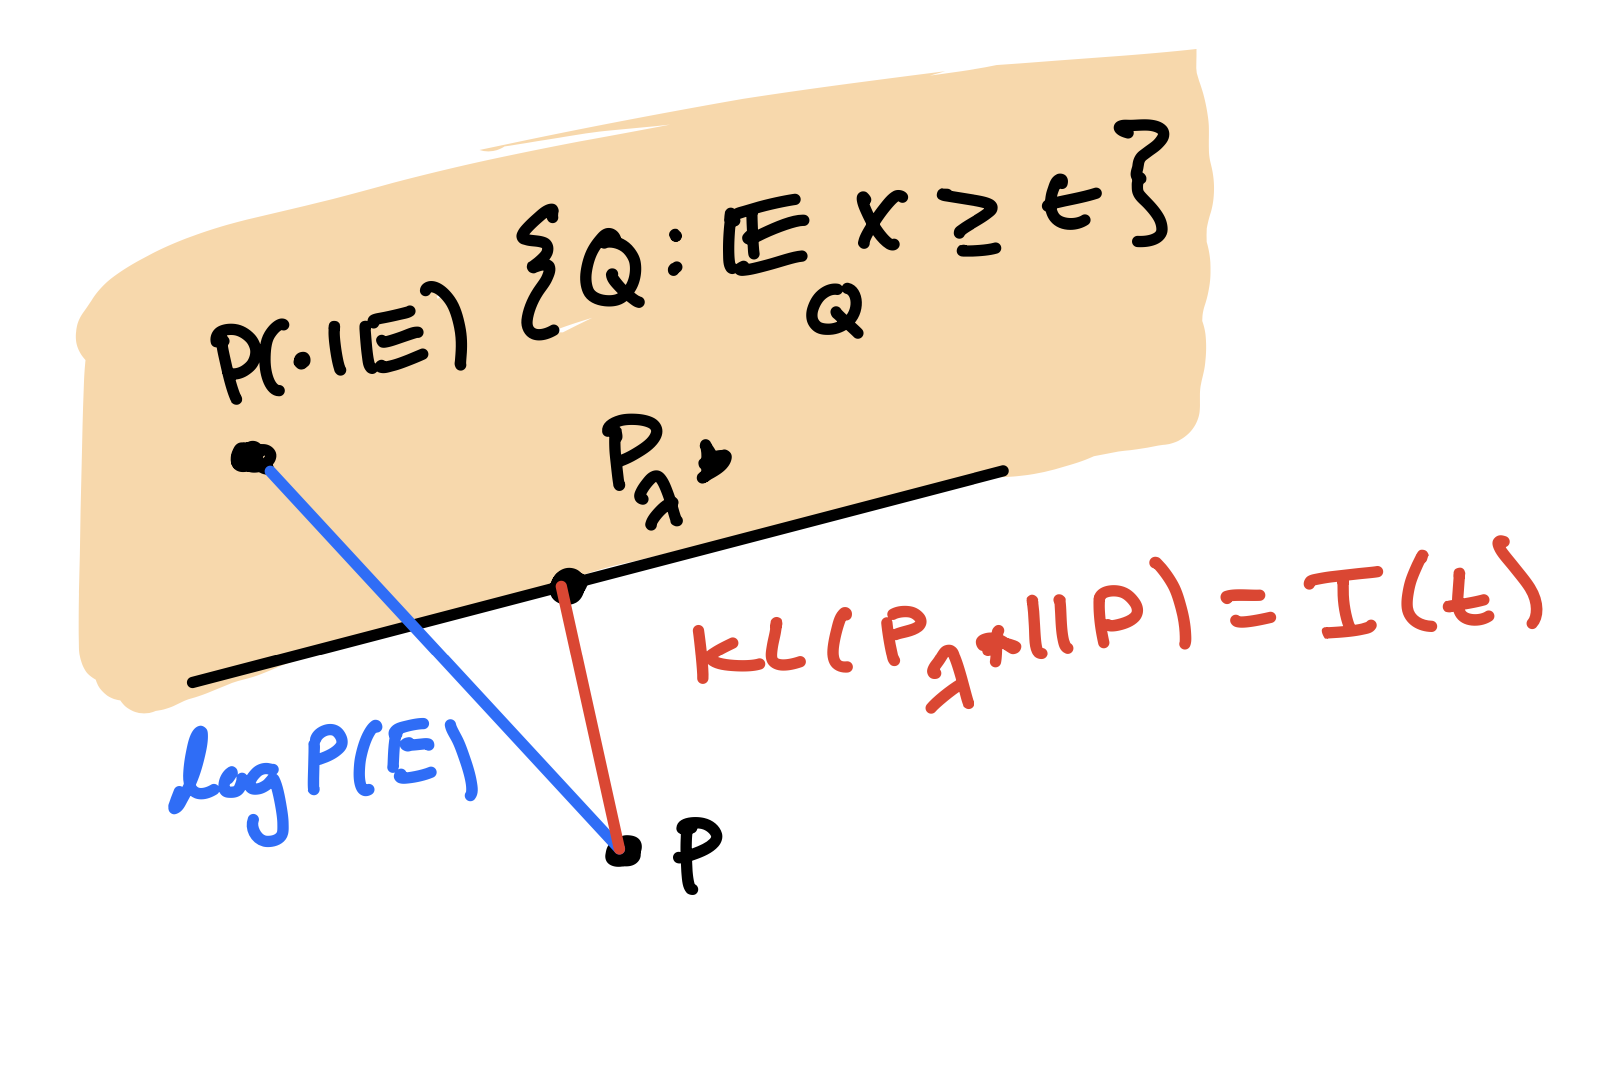
\includegraphics[width=5.20833in,height=\textheight,keepaspectratio]{project.png}

}

\caption{The KL projection of \(P\) onto the set of measures
\(\{Q \ : \ \E_Q[X] \geq t\}\) defines the rate function}

\end{figure}%

\subsubsection{Duality}\label{duality}

We've now motivated the Chernoff bound by (a) a numerical inequality (b)
a change of measure argument (c) a geometric argument in measure space.
These apparently distinct tricks are really just one -- an eccentric old
codger who wears many hats. We can expose his bald pate using the
language of duality.

The Legendre-Fenchel dual of a function \(f: V \rightarrow \mathbb{R}\),
where \(V\) is a real vector space, is defined as
\(f^*: V^* \rightarrow \mathbb{R}\) by \[
f^*(\lambda) = \sup_{x \in V} \langle \lambda, x \rangle - f(x)
\] where \(\lambda \in V^*\), the dual space of \(V\), and
\(\langle \lambda, x \rangle\) denotes the action of the linear
functional \(\lambda\) on \(x\). Intuitively, \(f^*(\lambda)\) gives the
maximal offset needed so that the affine functional
\(x \mapsto \langle \lambda, x \rangle - f^*(\lambda)\) lies below
\(f(x)\) everywhere. For convex \(f\), the biconjugate \(f^{**}\)
recovers \(f\), i.e., \(f^{**} = f\).

The fenchel duality principle says that (under mild conditions), if
\(f: V \rightarrow R\), \(g: W \rightarrow R\) are functions on vector
spaces \(V\) and \(W\), and \(A: V \rightarrow W\) is linear, then
\[\inf_{x \in V} f(x) + g(Ax) = \sup_{y \in W^*} -f^*(A^*y) - g^*(-y)\]

Where \(A^*\) is the adjoint of \(A\). Suppose we wish to handle the
constraint \((Ax)_i \geq t_i\). We can do this by defining
\(\iota_{t_i}(z) = \infty \times 1\{z \geq t_i\}\). We then have
\(\iota^*_{t_i}(y) = \sup_z z\times y - \iota(z) = \sup_{z \leq t_i} z \times y = t_i y\).

Let's make an observation here, so that we can instantiate this
machinery for our problem:

\textbf{(Donsker-Varadhan)} Let \(f\) be a function and \(X \sim P\).
Then \[\log \E \exp f(X) = \sup_Q \E_Q f(x) - KL(Q || P)\] \emph{Proof:}
Let \(P_f\) be such that \(dP_f/dP = e^{f(x)}/\E_P[e^{f(x)}]\)
\[\max_Q \E_Q[f(X)] - KL(Q || P) = \max_Q \E_Q[f(x)] - \E_Q[\log \frac{dQ}{dP_f}\frac{dP_f}{dP}]\]
\[= \max_Q \E_Q[f(x)] - KL(Q || P_f) - \E_Q[f(X)] + \log \E_P \exp f(X)\]
\[ = \max_Q \log \E_P \exp f(X) - KL(Q || P_f)\]

which is clearly achieved by \(Q = P_f\) and takes value
\(\log \E_P \exp f(X)\)

\emph{qed}

This is duality between the functionals
\(\Lambda(f) := (f \mapsto \log \E_P \exp f(X))\) and
\(KL(\cdot || P): Q \mapsto KL(Q || P)\), where measures \(Q\) act on
functions \(f\) via \(\langle Q, f\rangle := \E_Q f(X)\). Because
\(\Lambda(f)\) is convex, we have as a corollary
\[KL(Q || P) = \sup_f \E_Q[f(X)] - \Lambda(f)\]

This adds convex structure to the dualities between functions spaces and
measures spaces that are studied in analysis\footnote{To be concrete, we
  can take the set of measures to be those with densities wrt \(P\),
  which we can think about as the sphere in \(L^1(P)\). The dual
  variable then rightly in \(L^\infty(P)\). Then we denote
  \(\langle Q, f\rangle = \E_Q[f(X)]\).}, allowing us to associate a
function \(f\) with the measure that witnesses the supremum in
Donsker-Varadhan (and vice-versa).

\subsubsection{Coda: Chernoff again}\label{coda-chernoff-again}

Suppose we restrict ourselves to a finite list of test functions,
\(f_1, ... f_d\). Let us consider the following problem

\[\min_{Q \ \ \E_Q[f_i(X)] \geq t_i \ i = 1, ... d}KL(Q || P)\]

Let \(AQ = [\E_Q[f_1(X)], ... \E_Q[f_d(X)]]^T\). Its adjoint is
\(A^*: \lambda \mapsto \sum_i \lambda_i f_i\). By Fenchel duality, we
have that

\[\min_{Q \ \ \E_Q[f_i(X)] \geq t_i}KL(Q || P) = \min_Q KL(Q || P) + \sum_{i = 1}^d\iota_{t_i}(\E_Q[f_i(X)])\]
\[= \sup_\lambda - \Lambda(A^*\lambda) - \sum_{i = 1}^d \iota^*_{t_i}(\lambda_i)\]
\[= \sup_\lambda \lambda_i t_i - \log \E_P \exp{\sum_i \lambda_i f_i(X)}\]

So optimizing over an \(f\)-constrained set of measures in the primal
corresponds to optimizing the penalized CGF over the \(f\)-span in the
dual. In particular, our test functions define the constraints
\(\E_Q[f_i(X)] \geq t_i\) for \(i = 1, ..., d\). Let's call these
\(C_f\).

Recalling Proof 4, we can notice that as long as the conditional law
\(P(\cdot | E)\) lies in the constraint set, the projection
\(P^* = \min_{Q \in C_f}KL(Q || P)\) always defines an upper bound. By
adding more constraints to \(C_f\) that are satisfied by
\(P(\cdot | E)\), we make \(P^*\) closer to \(P(\cdot | E)\) and tighten
our bound. In the dual, this corresponds to finding the tightest upper
bound (in the \(L^1(P)\)-norm) to \(1\{x \geq t\}\) that is of the form
\(e^{\sum_{i = 1}^d f_i(x)}\).

\begin{figure}[H]

{\centering 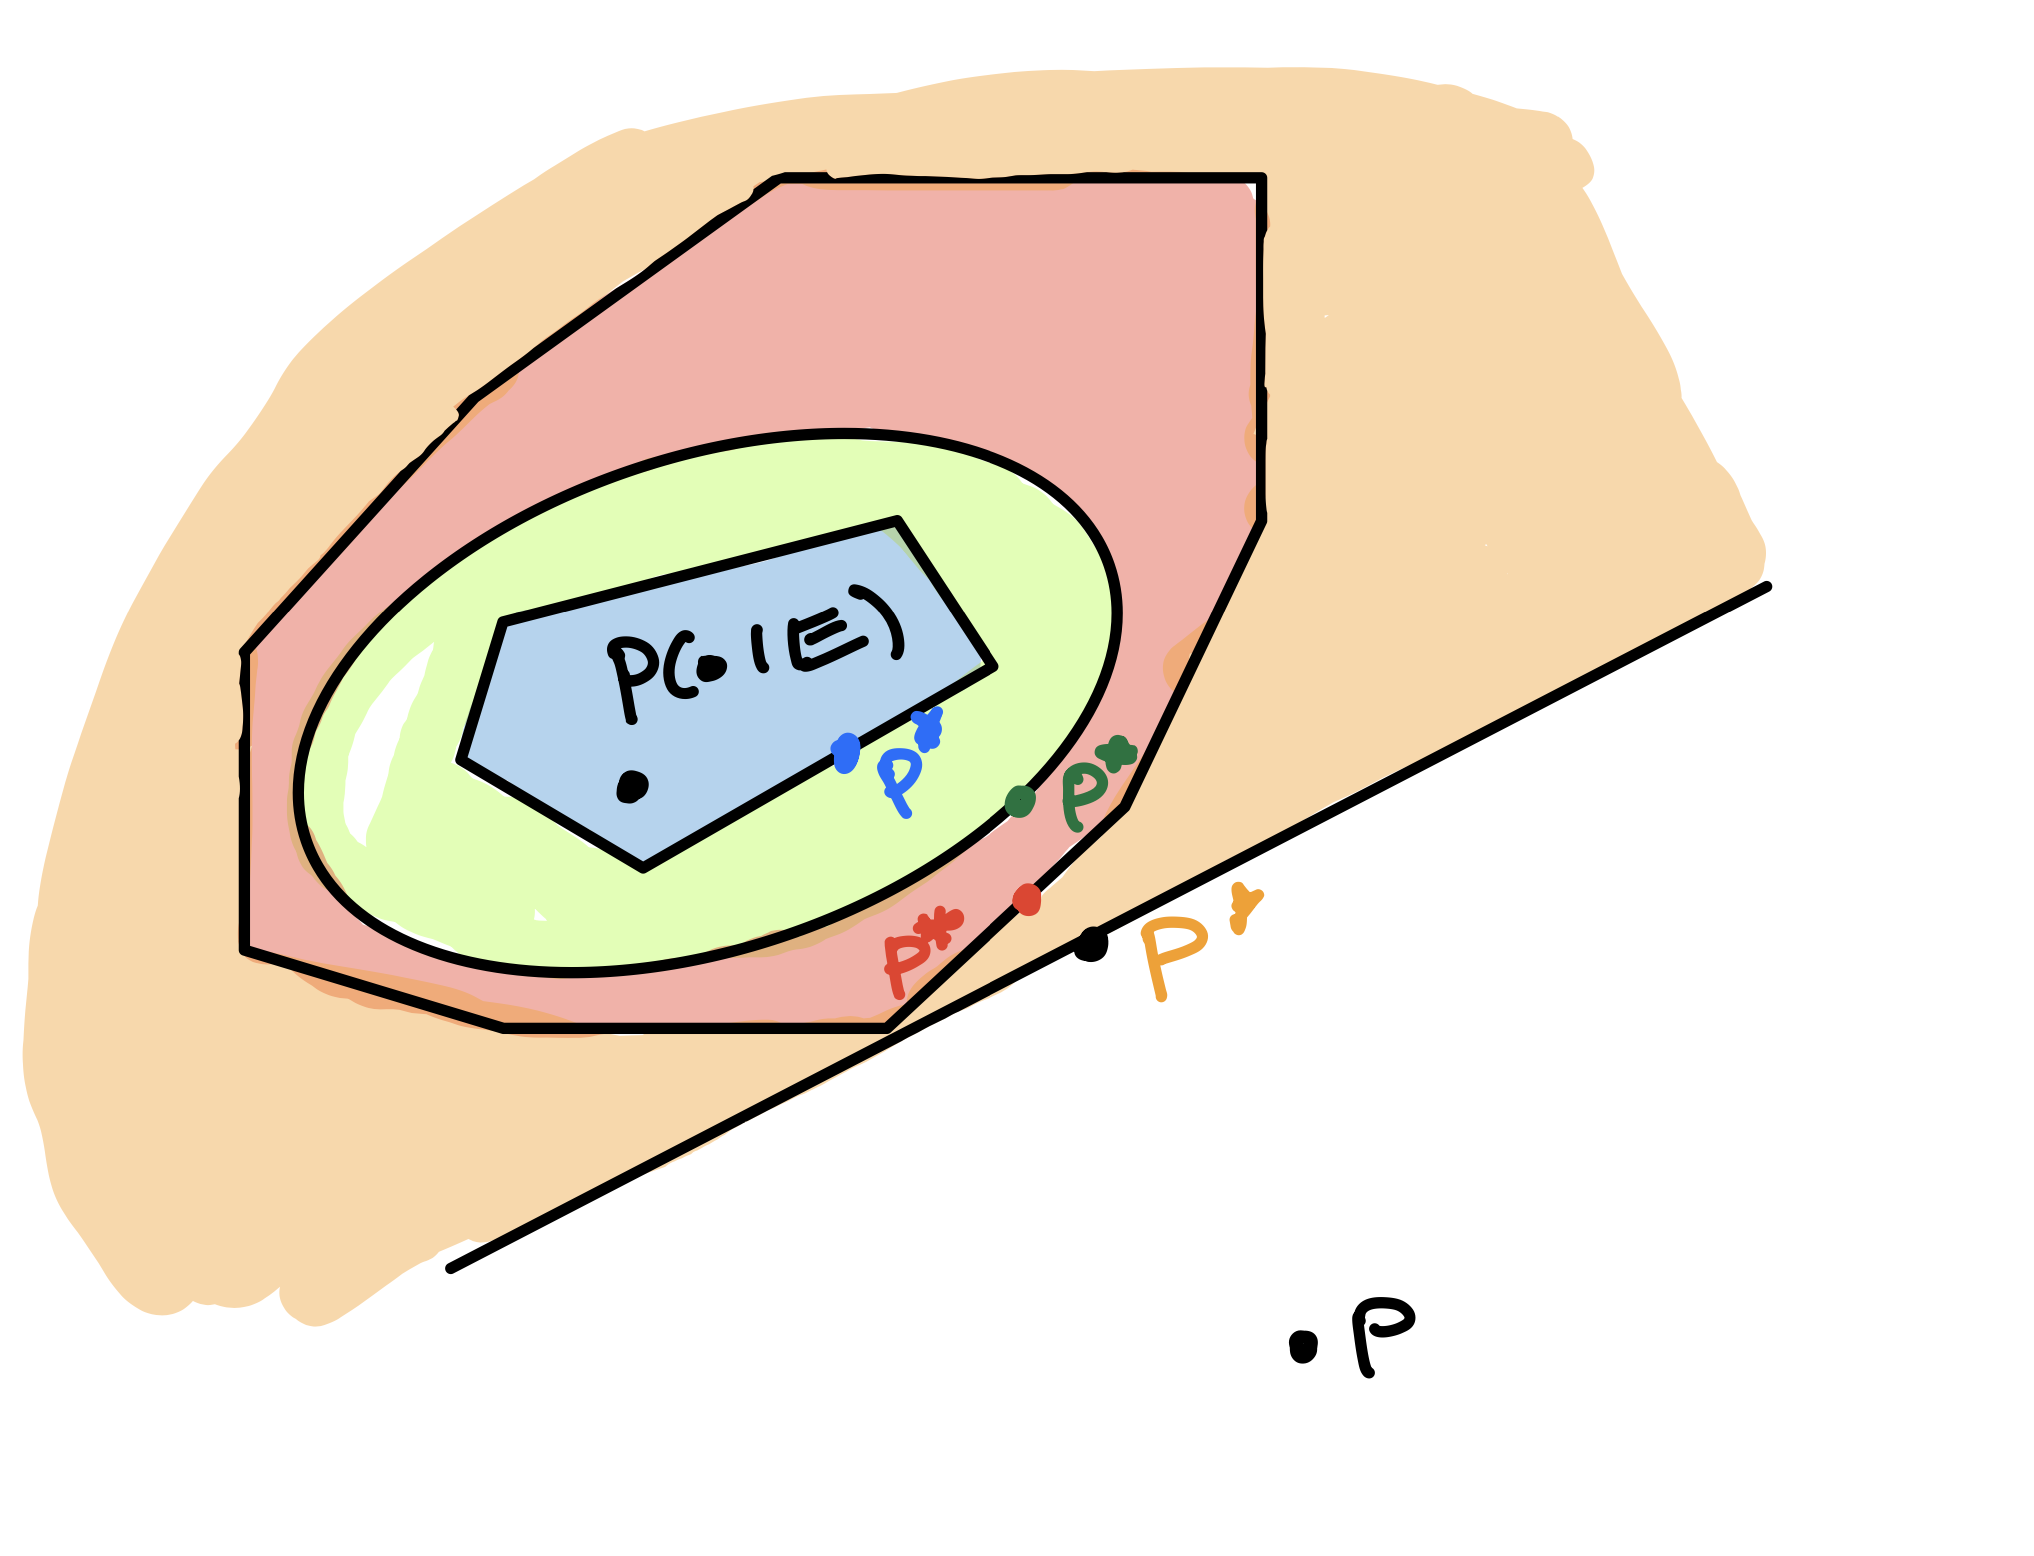
\includegraphics[width=5.20833in,height=\textheight,keepaspectratio]{many_constraint_sets.png}

}

\caption{As we add constraints that are satisfied by the conditional
law, \(P(\cdot | E)\), we tighten our approximation, at the cost of
making the bound less tractable. As we shall see in the next section, a
single linear constraint is asymptotically optimal, in the sense that
all other constraints that are satisfied by \(P(\cdot | E)\) will become
inactive as \(n \to \infty\).}

\end{figure}%

The Chernoff bound instantiates this machinery with just one, Spartan
test function: \(f_1(x) = x\), as we saw in Proofs 2, 3, and 4. As we
have already seen, optimizing over a single linear test function
corresponds to placing a single, linear mean constraint in measure
space. You can use Donsker-Varadhan to verify that the \(KL\) distance
from \(P(\cdot | E)\) to \(P_{\lambda^*}\) is exactly the \(L^1(P)\)
error of \(e^{\lambda^*(x - t)}\) against \(1\{x \geq t}\).

Why don't we use more test functions? This would make our approximation
\(P_f\) closer to \(P(\cdot | E)\). It turns out that a single linear
test-function is sufficient to get the right bound as \(n \to \infty\).
This is something we can intuit using the formulation from Proof 3.

\section{Lower bound}\label{lower-bound}

Let us now consider the tails of the random variable
\(X^n := \frac{1}{n}\sum_{i = 1}^n X_i\), and prove a lower bound that
says that we don't gain anything (asymptotically) by expanding our list
of test functions. We call \(X^n\)'s' law \(P_n\), derived from the
marginal law \(X \sim P\).

It's hard to get a lower bound out of the geometric perspective; the KL
divergence, ever indifferent to the axioms of distances, is more useful
for getting upper bounds. Therefore, we return to Proof 3 to show that
the change of measure argument is tight.

In particular, we'll gesture at Cramer's theorem, which says that if the
CGF is finite in a neighborhood of zero, then
\[\lim\sup \frac{1}{n} \log \Pr[X^n \geq t] = -I(t)\]

Let's just define \(A_n = \{X^n \in [t, t + \epsilon\}\) for some
\(\epsilon > 0\). Now, defining
\(P_{\lambda^* _n} = (P_{\lambda^*})^{\otimes n}\), we have

\[P_n(E) = \E_{P_n}[1\{A_n\}]\]
\[= \E_{P_{\lambda^*, n}}[e^{\lambda^* X_n - \psi_n(\lambda^*)}1\{A_n}]\]
\[\geq P_{\lambda^*_n}(A_n) \times  e^{\lambda^* (t + \epsilon) - \psi_n(\lambda^*)}\]
\[=  (\frac{1}{2} + o(1)) \times e^{-n I(t) + \lambda^* \epsilon}\]

where the final line holds by CLT applied to \(P_{\lambda^*, n}\). We
can now take \(\epsilon \downarrow 0\). In English, the Proof 3
perspective allows us to apply exact limit theorems to the tilted
distribution at the cost of the likelihood ratio evaluated within an
\(\epsilon\)-ball around \(t\). Shrinking the \(\epsilon\) makes the
likelihood ratio appraoch \(e^{-n I(t)}\).

\section{Next time}\label{next-time}

We'll see how algorithms for online prediction and boosting use nearly
the same procedures to get regret bounds in adversarial settings.




\end{document}
